\subsection{Histogram orientovaných gradientů HOG}

Základní myšlenkou je, že objekt v obraze může být pomocí vzhledu a tvaru charakterizován pomocí intenzity gradientů, i přestože neznáme jejich přesnou polohu v obraze. Autoři jsou N. Dalal a B. Triggs (2005).
\begin{enumerate}
  \item před započetím výpočtů je třeba normalizovat, například normalizaci barev a~gamy, v~případě černobílých obrázků k~normalizaci kontrastu (tento krok může být přeskočen,dle Dalal a~Triggs $\,\to\,$ předzpracování má malý vliv na výkon)
  \item obraz se \textbf{rozdělí} na malé prostorové oblasti (buňky, například $8 \times 8$ pixelů)
  \item pro každou buňku se vypočítá 1-D \textbf{histogram}, který je vypočítán ze všech pixelů z buňky (hodnoty buněk jsou rovnoměrně rozloženy do histogramu o~9 kanálech (binech) po \ang{20}; rozsah \ang{0}--\ang{180})  $\,\to\,$ výjde nám vektor o velikosti 9
  \item buňky spojíme do větších \textbf{propojených bloků} $16 \times 16$ z~důvodu normalizace osvětlení a~kontrastu. Pro chodce se používá L2--norm normalizace, dle vztahu \eqref{eq:normHog} $\,\to\,$ vznikne vektor velikosti $9\times4$ = 36 (čtyři $8 \times 8$ bloky)
  \item vektor normalizovaných histogramů pro jeden blok nazýváme \textbf{deskriptor}.
  \item spojíme tyto normalizované vektory do jednoho a získáme \uv{trénovací} vektor příznaků (features)
\end{enumerate}
Existují dvě varianty spojení bloků, tzv. obdélníkové bloky (R--HOG) a~kruhové bloky (C--HOG).
Rozdělení do rozsahu 0--\ang{180} proto, že se jedná o bezznaménkové gradienty (unsigned) a bylo dokázáno, že fungují lépe než znaménkové (signed) 0--\ang{360}. Některé implementace HOG umožní určit, zda chceme používat signed gradienty.
\begin{equation}
\centering
 \label{eq:normHog}
 \begin{aligned}
L2-norm&: \qquad  f =& \frac{v}{\sqrt{\lVert v~\lVert_2^2 + e^2}} \\
L1-sqrt&: \qquad  f =& \sqrt{\frac{v}{\lVert v~\lVert_1 + e}}
 \end{aligned}
\end{equation}
Nechť $v$ je nenormalizovaný vektor obsahující všechny histogramy v~daném bloku, $\lVert v~\lVert_k$ je jeho k--norm pro $k = 1,2$, a~$e$ je malá konstanta.

\textbf{C--HOG} (Kruhové HOG bloky) - lze nalézt ve dvou variantách: \textit{s~jedinou, centrální buňkou} a~\textit{úhlově rozdělenou centrální buňkou}. Dají se popsat čtyřmi parametry: počtem úhlů a~radiálních kanálů (binů), poloměrem centrálního binu a~faktorem roztažení pro poloměr dalších radiálních binů.

\textbf{R--HOG} (Obdélníkové HOG bloky) - tyto bloky jsou v~praxi nejčastěji používané a~reprezentují se třemi parametry: \textit{počet buněk na blok}, \textit{počet pixelů na buňku} a~\textit{počet binů (kanálů) na jeden histogram}. R--HOG bloky se také používají pro kódování informací. 
\begin{figure}[H]
  \centering
  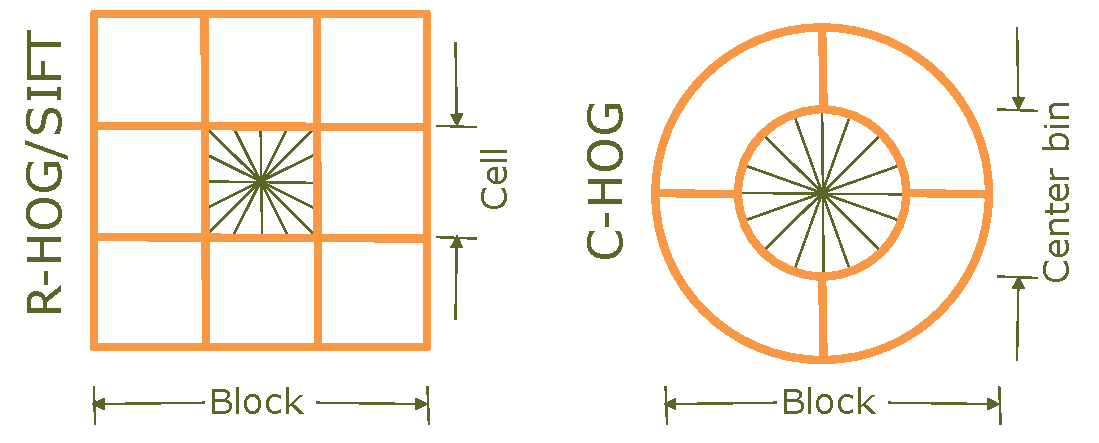
\includegraphics[width=10cm]{assets/9_hog_variants.pdf}
  \caption{Varianty geometrie spojení bloků}
  \label{variants_block}
\end{figure}

\subsection{SIFT/SURF - detektory a popisovače klíčových bodů}
Využívá se stejný princip tvoření histogramu jako u metody HOG
\begin{itemize}
\item klíčové body jsou nezávislé na osvětlení, velikosti, orientaci, pozici
\item Octave - úroveň skálování
      \begin{itemize}
          \item 4 oktávy a 5 rozmazání “ideál” dle prezentace, každá oktáva se 5x rozmaže
          \item vypočítá se rozdíl mezi rozmazanými obrázky
          \item klíčový bod najdeme jako minimum/maximum mezi ruznými urovněmi rozmazání 
      \end{itemize}
  \item poté musíme provést eliminaci slabých bodů
      \begin{itemize}
          \item odebereme ty s malou intenzitou
          \item odstraníme klíčové body, které leží na hraně - využit princip Harrisova detektoru hran - Hessian matice (matice druhých derivací)
      \end{itemize}
  \item orientace bodu se vypočítá pomocí histogramu směrů gradientů v okolních bodech, zajišťuje nám to invarianci vůči rotaci (36 košů)
  \item Descriptor
      \begin{itemize}
          \item 16x16 matice okolo klíčových bodů 
          \item rozdělit na 4x4 subbloky (16 bloků v 16x16 okolí)
            \begin{itemize}
                \item v nich vypočítat histogram orientací gradientu
                \item poté tento histogram převést do vektoru (viz HOG)
                \item spojit pro všechny bloky a máme výsledný vektor
            \end{itemize}
      \end{itemize}
  \item SURF má stejné kroky jako SIFT, jen má jiné \uv{implementace} kroků
\end{itemize}

\subsection{Haarovy příznaky}
\begin{itemize}
  \item Na tomto přístupu je založen objektový detektor \textbf{Viola--Jones} (\textit{Viola--Jones object detector framework}).
  \item Poskytuje v~reálném čase \textbf{spolehlivou} a~\textbf{konkurenceschopnou} detekci objektů.
  \item Může být vytrénován pro detekci různých objektových tříd (primárně určen pro \textbf{detekci obličejů}).
  \item Detektor pracuje s~obrazy ve stupních šedi a~skládá se ze tří částí. (Integrální obraz, Haar příznaků a~AdaBoost algoritmus)
\end{itemize} 
Integrální obraz je takový obraz (obrázek \ref{fig:integralimage}), kde každý bod $x$ představuje součet hodnot předchozích pixelů doleva a~nahoru. Spodní pravý bod obsahuje součet všech pixelů v~obraze.
Zápis integrálního obrazu je:
\begin{equation*}
\label{integralimage}
 I(x, y) = \sum_{\substack{x' \leq x \\ y' \leq y}}{} i(x', y'),
\end{equation*}
kde $i(x', y')$ je hodnota pixelu na pozici $(x, y)$.
\begin{figure}[H]
\centering
\begin{minipage}{.4\textwidth}
  \centering
  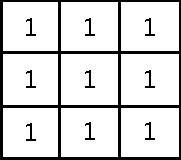
\includegraphics[width=.5\linewidth]{assets/9_ii_input}
  \caption{Vstupní obraz}
  \label{fig:ii_input}
\end{minipage}%
\begin{minipage}{.4\textwidth}
  \centering
  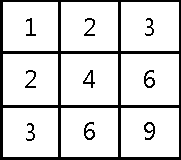
\includegraphics[width=.5\linewidth]{assets/9_ii_output}
  \caption{Integrální obraz}
  \label{fig:ii_output}
\end{minipage}
\caption{Převod obrazu na integrální obraz}
\label{fig:integralimage}
\end{figure}

Princip využití Haarových příznaků v~obrazech je založen na pozorování, že lidská těla a~obličeje mají některé podobné rysy. Právě tyto rysy mohou být porovnány pomocí Haarových příznaků. Jedná se například o~tyto rysy:
\begin{itemize}
  \item{Oční oblast je tmavší než oblast nosního mostu,}
  \item{hlava člověka je tmavší než její okolí,}
  \item{oblast mezi dolními končetinami je světlejší než samotné nohy.}
\end{itemize}
Sada Haarových vlnek je na obrázku \ref{fig:basichaarfeatures}, jedná se pouze o~základní sadu příznaků.
\begin{figure}[H]
\centering
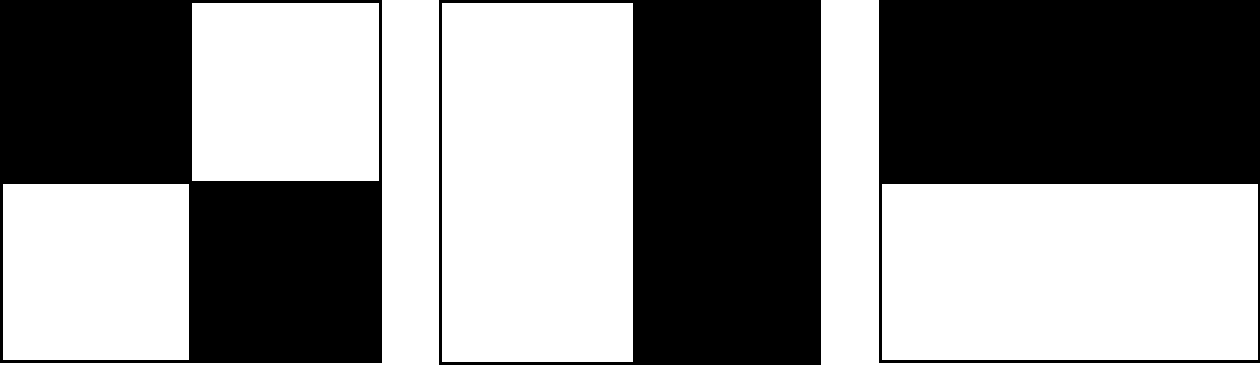
\includegraphics[width=.4\linewidth]{assets/9_haar_features}
\caption{Základní sada Haarových příznaků}
\label{fig:basichaarfeatures}
\end{figure}

Pro identifikaci lidských postav se používá rozšířená sada vlnek, tzv. Haar--like příznaky. Klasifikační systém založený na těchto Haar--like příznacích dosahuje nižší falešně pozitivní detekce než původní Haar příznaky. Na obrázku \ref{fig:haarlike} je příklad detekce pomocí Haar--like vlnek. Hodnota příznaku je rozdíl mezi sumou hodnot pixelů v~bílé a~černé oblasti Haarových vlnek.
\begin{figure}[H]
\centering
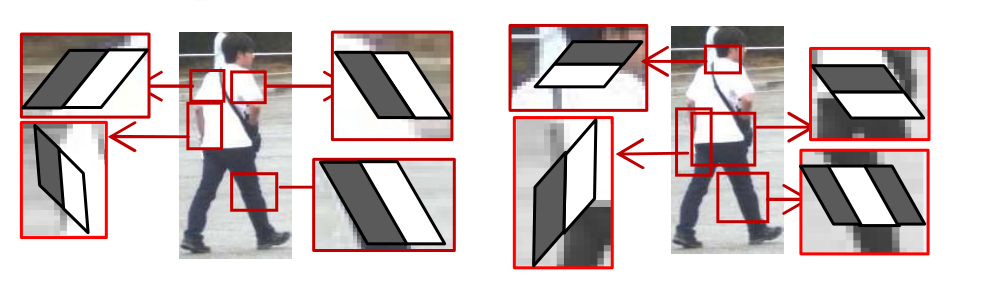
\includegraphics[width=.8\linewidth]{assets/9_haar-like}
\caption{Použití Haar--like příznaků na chodcích}
\label{fig:haarlike}
\end{figure}

\subsection{LBP Lokální binární vzor}
Hlavní myšlenkou LBP je, že struktury obrazu mohou být efektivně zakódovány porovnáním hodnot jednotlivých pixelů a~jejich okolí. Tato metoda je odolná vůči jasovým změnám obrazu.
\begin{enumerate}
  \item převod obrazu do stupňů šedi a~jeho rozdělení do buněk
  \item okolní hodnoty pixelů jsou porovnávány se středovým pixelem, pokud je jejich hodnota rovna nebo větší zapíše se na tuto pozici jednička v~opačném případě nula
  \item tyto hodnoty seřadíme dle hodinových ručiček nebo naopak a~získáme osmimístné binární číslo a převedeme do dekadické soustavy
  \item z~čísel, které jsme získali kombinací pixelů v~buňkách, vypočítáme histogram
  \item zřetězíme všechny histogramy buněk a~získáme vektor příznaků pro celý obraz (jedná se o~256--dimenzionální vektor příznaků)
\end{enumerate}
Matematicky lze LPB vyjádřit jako:
\begin{equation*}
LBP_{P,R} = \sum_{p=0}{P-1} s(g_p - g_c)2^P, \\
s(x) =
  \begin{cases} 
   1 & \text{pro } x \geq 0, \\
   0       & \text{pro } x < 0,
  \end{cases}
\end{equation*}
kde: $P$ je počet bodů v~okolí, $R$ vyjadřuje vzdálenost bodů od středového pixelu, $g_c$ je středový pixel, $g_p$ je aktuální pixel. 

Následující příklad se vztahuje k~obrázku \ref{fig:lbpsum}. Po porovnání pixelů se středovým pixelem jsme získali vzor $11110001$. Tento vzor převedeme do dekadické soustavy a~sečteme, $ 1+16+32+64+128 = 241$. Získali jsme hodnotu této buňky do vektoru příznaků.

\begin{figure}[H]
\centering
\begin{minipage}[b]{.3\textwidth}
  \centering
  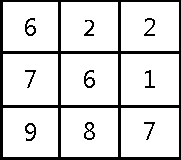
\includegraphics[width=.5\linewidth]{assets/9_lbp_img}
  \caption*{Vstupní buňka}
  \label{fig:lpbimg}
\end{minipage}%
\begin{minipage}[b]{.3\textwidth}
  \centering
  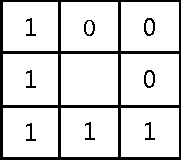
\includegraphics[width=.5\linewidth]{assets/9_lbp_thresh}
  \caption*{Prahové hodnoty}
  \label{fig:lbpthresh}
\end{minipage}
\begin{minipage}[b]{.3\textwidth}
  \centering
  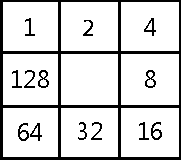
\includegraphics[width=.5\linewidth]{assets/9_lbp_weights}
  \caption*{Pixely ohodnoceny váhou}
  \label{fig:lbpweights}
\end{minipage}
\caption{Výpočet příznaku}
\label{fig:lbpsum}
\end{figure}

Výhoda této metody je její rychlý a~snadný výpočet a~odolnost vůči různým osvětlením. Na druhou stranu je těžší na trénování, protože výsledné dekadické číslo může mít obrovské množství možností (podle parametru $P$). K~omezení lze využít uniformní vzory (obrázek \ref{fig:lbpvzory}). Pro parametr $P=8$, získáme 59 vzorů. 

\begin{figure}[H]
\centering
\begin{minipage}[b]{.18\textwidth}
  \centering
  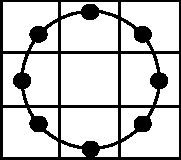
\includegraphics[width=.9\linewidth]{assets/9_lbp_spot}
  \caption*{Bod}
\end{minipage}
\begin{minipage}[b]{.18\textwidth}
  \centering
  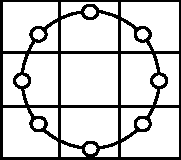
\includegraphics[width=.9\linewidth]{assets/9_lbp_spot_flat}
  \caption*{Bod/Plocha}
\end{minipage}
\begin{minipage}[b]{.18\textwidth}
  \centering
  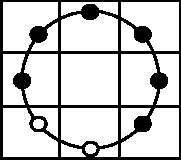
\includegraphics[width=.9\linewidth]{assets/9_lbp_line}
  \caption*{Křivka}
\end{minipage}
\begin{minipage}[b]{.18\textwidth}
  \centering
  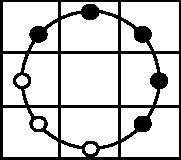
\includegraphics[width=.9\linewidth]{assets/9_lbp_corner}
  \caption*{Roh}
\end{minipage}
\begin{minipage}[b]{.18\textwidth}
  \centering
  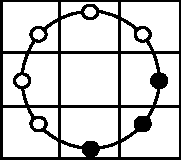
\includegraphics[width=.9\linewidth]{assets/9_lbp_edge}
  \caption*{Hrana}
\end{minipage}
\caption{Lokální okolí LBP metody}
\label{fig:lbpvzory}
\end{figure}

\subsection{Klasifikátory}
Klasifikace je obecný proces kategorizující objekty do určitých tříd. Termín klasifikátor někdy odkazuje také na matematickou funkci, implementovanou klasifikačním algoritmem.
\subsubsection*{SVM Support vector machines} % @TODO
\begin{itemize}
  \item První algoritmus přisuzován Vladimíru Vapnikovi (1963)
  \item Učební modely, které jsou velmi populární v~oblasti strojového učení.
  \item Založena na tzv. \textbf{jádrových algoritmech} (kernel machines) s~využitím \textbf{podpůrných vektorů} (support vectors).
  \item Původně tato technika sloužila k~vytvoření optimálního binárního klasifikátoru, později byla rozšířena na řešení \textbf{problému regrese} a~\textbf{shlukování}.
  \item Byly úspěšně použity ve třech hlavních oblastech: kategorizace textu, rozpoznání obrazu a~bioinformatika (např. třídění novinových zpráv, rozpoznávání ručně psaných čísel nebo například vzorky rakovinových tkání).
\end{itemize}

Primárním cílem SVM je nalézt \textbf{nadrovinu}, která \textbf{optimálně rozděluje prostor} příznaků tak, aby trénovací data náležela do konkrétních tříd. Tuto nadrovinu ilustruje obrázek \ref{fig:svm}. Pokud mezera mezi oddělující nadrovinou a~nejbližšími vektory příznaků z~obou kategorií (v~případě binárního klasifikátoru) je maximální, jedná se o~optimální řešení. Vektory příznaků v~blízkosti této nadroviny se nazývají podpůrné vektory, což znamená, že pozice ostatních vektorů nemá vliv na nadrovinu (rozhodovací funkce). 

Jinými slovy, se jedná o~diskriminační klasifikátor formálně definovaný rozdělovací nadrovinou, která kategorizuje nové příklady.
\begin{figure}[H]
\centering
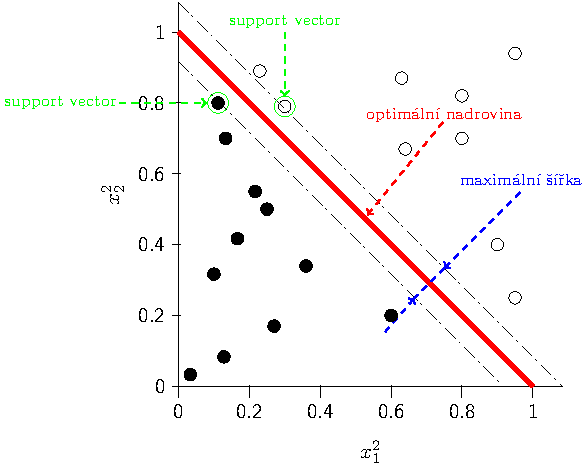
\includegraphics[width=.71\linewidth]{assets/9_svm.pdf}
\caption{Optimální oddělovací hranice}
\label{fig:svm}
\end{figure}

Implementaci SVM lze nalézt v~již existujících knihovnách, jako jsou například LIBSVM, kernlab, scikit-learn, SVMLight.. 
\begin{itemize}
\item\textbf{$C$--Support vektorová klasifikace ($C$--SVC)} -- 
Umožnuje nedokonalé oddělení tříd pro $n$--tříd ($n > 2$) s~postihovým multiplikátorem $C$, pro odlehlé hodnoty ($C > 0$).
\item\textbf{$\nu$--Support vektorová klasifikace ($\nu$--SVC)} --
$n$--třídní klasifikace s~možností nedokonalé separace. Tato klasifikace přidává nový parametr $\nu \in (0;1\rangle$, čím větší je jeho hodnota, tím hladší je rozhodovací funkce. 
\item\textbf{Distribuční odhad (Jednotřídní SVM)} --
Distribution Estimation (One-class SVM), jak již název sám o~sobě napovídá všechny trénovací data pocházejí z~jedné třídy, SVM vytvoří hranici, která odděluje třídu od zbývající části.
\item\textbf{$\varepsilon$--Support vektorová regrese ($\varepsilon$--SVR)} --
Vzdálenost mezi vektory příznaků a~rozdělovací nadrovinou musí být menší než mez tolerance $\varepsilon$. Pro odlehlé hodnoty opět použijeme multiplikátor $C$. Musí tedy platit: $C > 0$ a~$\varepsilon > 0$. 
\item\textbf{$\nu$--Support vektorová regrese ($\nu$--SVR)} --
Tato klasifikace je podobná jako $\varepsilon$--SVR. Na místo $\varepsilon$ se použije parametr $\nu \in (0;1\rangle$. 
\end{itemize}
Účinnost SVM závisí na výběru správného jádra a~jeho parametrů. Často se používá Gaussovo jádro s~jedním parametrem $\gamma$. Díky jeho přesnosti, ale je časově náročné. V~této knihovně se můžeme setkat s~následujícími jádry.
\begin{itemize}
\item\textbf{Lineární jádro} --
Použití tohoto jádra je velmi rychlé (bez jakékoliv transformace), jedná se o~lineární diskriminaci a~rozdělovací nadrovina bude vždy přímka. Pro toto jádro platí 
\begin{equation*}
 \label{linearK}
  K(x_i, x_j) = x_i^T x_j,
\end{equation*}
  kde $x_i$ a~$x_j$ jsou vektory vstupního prostoru.

\item\textbf{Polynomické jádro} --
Polynomické jádro umožňuje učení nelineárních modelů
\begin{equation*}
\label{polyK}
  K(x_i, x_j) = (\gamma x_i^T x_j + c)^{d}, \gamma > 0,
\end{equation*}
kde: $c \geq 0$, volný parametr, který vylučuje vliv vyššího řádu oproti polynomu nižšího řádu (pokud $c = 0$, jádro je homogenní), řád polynomu určuje parametr $d$.

\item\textbf{Gaussovo jádro} --
Gaussovo neboli RBF (Radial Basis Function) jádro se řadí mezi nejpoužívanější a~je definované jako
\begin{equation*}
\label{RBFK}
 K(x_i, x_j) = e^{-\gamma ||x_i - x_j||^2}, \gamma > 0,
\end{equation*}
kde: $||x_i - x_j||^2$ značí kvadratickou euklidovskou vzdálenost mezi dvěma vektory příznaků.

\item\textbf{Sigmoidní jádro} --
toto jádro je podobné sigmoidní funkci v~logistické regresi
\begin{equation*}
\label{sigmK}
 K(x_i, x_j) = \tanh(\gamma x_i^T x_j + r),
\end{equation*}
kde $r$ je volitelný parametr.

\item\textbf{Exponenciální jádro} --
Exponenciální jádro $\chi$2 je podobné RBF jádru a~využívá se převážně na histogramy
\begin{equation*}
\label{expK}
 K(x_i, x_j) = e^{-\gamma \chi^2(x_i,x_j)}, \chi^2(x_i,x_j) = \frac{(x_i-x_j)^2}{(x_i+x_j)}, \gamma > 0,
\end{equation*}

\item\textbf{Jádro histogramu průsečíků} --
Toto jádro je také známé jako \textit{Min Kernel}, jedná se o~nejnovější jádro v~této knihovně a~je velmi rychlé a~užitečné při klasifikaci
\begin{equation*}
\label{innK}
 K(x_i, x_j) = min(x_i,x_j).
\end{equation*}
\end{itemize}

\subsubsection{KNN - K-nearest neighbours}
\begin{itemize}
\item velmi rychlý, jednoduchý
\item pomocí k sousedů určíme label dotazovaného 
\item pokud bereme v potaz jejich vzdálenosti jedná se o modifikované KNN
\item učení je velmi rychlé (jen se uloží data do struktur)
\item určení se zpomaluje se zvyšujícím se k
\end{itemize}

\subsubsection{Kaskádové klasifikátory} % @TODO
\begin{itemize}
  \item Skládá \textbf{z~více slabších} klasifikátorů umístěných v~\textbf{kaskádách} za sebou.
  \item Požadavky na tento druh klasifikátoru byly \textbf{rychlost} detekce, aby mohl být implementován na procesorech s~nižším výkonem. (v kamerách, v telefonech..)
  \item Klasifikátory si mezi sebou \textbf{předávají všechny} informace o~vstupním obraze (může se redukovat čas, nutný pro detekci v~daném obraze).
  \item Prvním takovým klasifikátorem byl detektor obličeje \textbf{Viola--Jones}
\end{itemize}
Klasifikátor na první vrstvě může vyfiltrovat většinu negativních oken. Na druhé vrstvě se mohou odfiltrovat \uv{těžší} negativní okna, která přežila z~první vrstvy a~tak dále. Subokno, které přežije všechny vrstvy, bude označeno jako pozitivní detekce. Příklad řetězce kaskádového klasifikátoru je ilustrován na obrázku \ref{fig:ccpipeline}, kde $K1$--$KN$ je klasifikátor první až $n$--té vrstvy.

\begin{figure}[H]
\centering
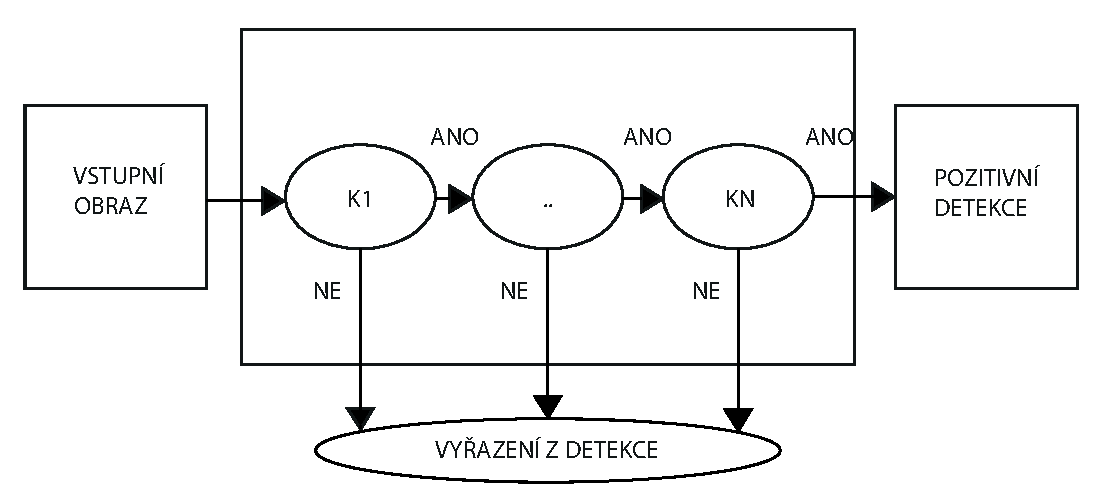
\includegraphics[width=.6\linewidth]{assets/9_cascadeClass.pdf}
\caption{Ukázka pipeline kaskádového klasifikátoru}
\label{fig:ccpipeline}
\end{figure}

\subsubsection{AdaBoost}
\begin{itemize}
  \item \textbf{AdaBoost}, neboli Adaptive Boosting
  \item klasifikátor \textbf{kombinuje} slabé klasifikátory k~vytvoření jednoho silného klasifikátoru
\end{itemize}
V~kombinaci více klasifikátorů s~výběrem trénovací sady v~každé iteraci algoritmu a~přidělení správné váhy na konci trénování, docílíme klasifikátoru s~dobrou přesností. Klasifikátory v~tomto řetězci, které mají klasifikační přesnost menší než 50\%, jsou ohodnoceny zápornou vahou. Váhou nula jsou ohodnoceny klasifikátory, které mají přesnost 50\%. Pouze ty, keré mají přesnost vyšší než 50\%, jsou přínosné do této kombinace a~můžeme hovořit o~zesílení (boosting) klasifikace. 

\subsection{Template Matching}
\begin{itemize}
\item vytvoříme si model objektu obsahující tvar, barvu a texturu 
\item následně se hledají v obraze jednotlivé prvky objektu samostatně a zjišťuje se míra podobnosti s vytvořeným modelem a tu pak v obrázku hledáme (pixel po pixelu)
\end{itemize}
Jednoznačnou výhodou tohoto přístupu je snadná implementace, ukázalo se však, že pro detekci obličejů není vhodná zdůvodů nízké odolnosti proti variabilitě
Změna velikosti, pozice nebo tvaru objektu významně ovlivňuje výsledky metody. 

Druhy metod:
\begin{itemize}
\item \textbf{SAD} suma absolutních rozdílů (Sum of Absolute Difference) --  lze vypočítat získáním absolutních rozdílů napříč všemi pixely mezi vstupním obrazem S a odpovídající pozicí pixelu v templatu T. Sumu těchto hodnot lze následně použít jako koeficient míry podobnosti mezi obrázkem S a templatem T, kdy čím menší tato hodnota je, tím více se jednotlivé pixely na daných pozicích shodují. Tudíž lze předpokládat, že se zde nachází hledaný objekt. 
\begin{figure}[H]
\centering
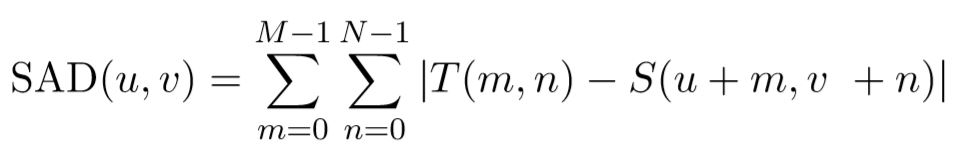
\includegraphics[width=.6\linewidth]{assets/9_sad}
\end{figure}
Ve srovnání s ostatními metodami (SSD, NCC) je SAD přímočará, jednoduchá a výpočetně nenáročná. Může být však nespolehlivá a produkovat chybné výsledky v případě změn ve světelných podmínkách, barvě, velikosti či tvaru. Díky své rychlosti je však možné ji použít spolu s jinými metodami, jako je detekce hran, pro zlepšení spolehlivosti.
\item \textbf{SSD} suma čtvercových rozdílů (Sum of Squared Difference) --  představuje jednu z více používaných metod pro výpočet koeficientu míry podobnosti. Nejmenší hodnota pixelu opět představuje nejlepší shodu, jako tomu bylo v případě SAD.
\begin{figure}[H]
\centering
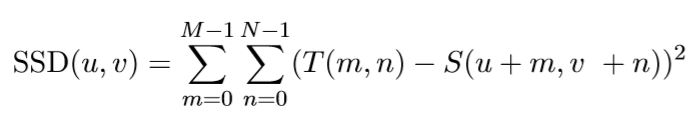
\includegraphics[width=.6\linewidth]{assets/9_ssd}
\end{figure}
Ve srovnání s SAD se jedná o výpočetně náročnější, z důvodů nutnosti násobení, ale stále velice používanou metodu. Převážně vzhledem ke své jednoduchosti a stále relativně malé výpočetní náročnosti. NCC však ve většině případů produkuje přesnější a spolehlivější výsledky.
\item \textbf{CC} vzájemná korelace (Cross-Correlation) --  představuje sumu párových násobků hodnot jednotlivých pixelů.
\begin{figure}[H]
\centering
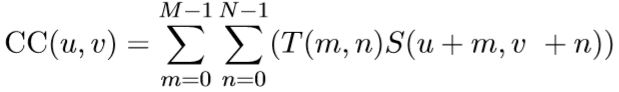
\includegraphics[width=.6\linewidth]{assets/9_cc}
\end{figure}
V reálných aplikacích se však tato metoda většinou nepoužívá. Přestože je relativně výpočetně nenáročná, tak vzhledem k její nespolehlivosti v případech, kdy se v obrázku nachází větší změny v měřítku nebo rotaci mezi hledaným objektem a vstupním obrazem, se využívá spíše její normalizovaná varianta, a to i přes daleko větší výpočetní náročnost.

\item \textbf{NCC} normalizovaná vzájemná korelace (Normalized Cross-Correlation) -- představuje jednu z nejpoužívanějších metod pro výpočet míry podobnosti mezi dvěma obrazy. Její největší výhodou oproti typické CC je větší odolnost vůči změnám v osvětlení scény.
\begin{figure}[H]
\centering
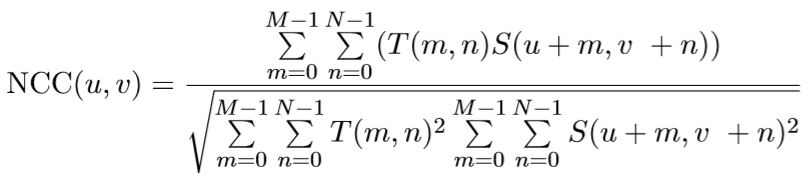
\includegraphics[width=.6\linewidth]{assets/9_ncc}
\end{figure}
V porovnání s metodami SAD, SSD a CC je NCC ve většině situací nejpřesnější, avšak výpočetně mnohem náročnější. Při jejím použití je, pro urychlení výpočtu koeficientů, doporučeno provést jednoduché předfiltrování zpracovávaných oken např. aplikací kontroly salience.
\end{itemize}
Všechny výše zmíněné metody bohužel trpí stejnými nedostatky. Při vyhledávání jsou výskyty vzorků ve vstupním obraze nuceny zachovat orientaci referenčního obrázku. Zároveň je velice neefektivní a časově náročné počítat korelaci mezi templatem a vstupním obrazem pro obrazy středních avyšších rozlišení.

\subsection{Deep learning}
\begin{itemize}
  \item Deep learning neboli \textbf{hluboké učení}, známé také jako hierarchické učení, je \textbf{sbírka algoritmů} používaných ve strojovém učení.
  \item Používají se k~modelování abstrakcí na vysoké úrovni v~datech za pomocí modelových architektur, které se skládají z~několika nelineárních transformací.
  \item Hluboké učení je součástí široké skupiny metod používané pro strojové učení, které jsou založeny na učení reprezentace dat.
\end{itemize}
Hluboké strukturované učení může být:
\begin{itemize}
  \item{\textbf{Kontrolované (s~učitelem)} - všechna data jsou kategorizovaná do tříd, algoritmy se učí předpovídat výstup ze vstupních dat.}
  \item{\textbf{Částečně kontrolované} - data jsou částečně kategorizovaná do tříd. Pří tomto přístupu učení lze využít kombinaci kontrolovaného a~nekontrolovaného přístupu učení.}
  \item{\textbf{Nekontrolované (bez učitele)} - data nejsou kategorizovaná do tříd, algoritmy se učí ze struktury vstupních dat.}
\end{itemize}
Hluboké učení je specifický přístup, použitý k~budování a~učení neuronových sítí, které jsou považovány za velmi spolehlivé rozhodovací uzly. Jestliže vstupní data algoritmu procházejí řadou nelinearit a~nelineárních transformací, tak tento algoritmus je považován za \uv{deep} algoritmus. 

Odstraňuje také ruční identifikaci příznaků (obrázek \ref{fig:ml_vs_ann}) z~dat a~místo toho se spoléhá na jakýkoliv trénovací proces, které má za úkol zjistit užitečné vzory ve vstupních příkladech. To dělá neuronovou síť jednodušší a~rychlejší, a~může přinést lepší výsledky než z~oblasti umělé inteligence.

\begin{figure}[H]
\centering
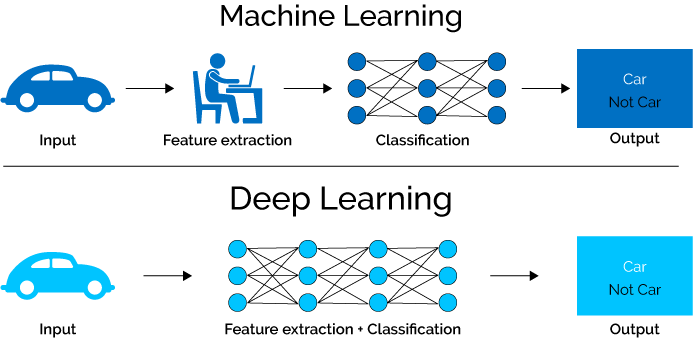
\includegraphics[width=.85\linewidth]{assets/9_ml_vs_ann}
\caption{Hlavním rozdílem mezi strojovým a~hlubokým učením je ten, že u~strojového se příznaky musí extrahovat manuálně. \cite{fig:mlvsann}}
\label{fig:ml_vs_ann}
\end{figure}

\subsubsection{Neuronové sítě \textit{ANN} - Artificial Neural Network}
\begin{itemize}
  \item Inspirované \textbf{lidským mozkem}, který je složený z~různých vzájemně propojených vrstev neuronů, kde každý z~nich přijímá informaci z~předchozího, zpracovává tuto informaci a~odesílá jí do dalšího neuronu, dokud není přijat konečný výstup.
  \item Může se jednat o~výstup \textbf{s~danou kategorií}, jestliže se jedná o~kontrolované učení nebo \textbf{o~určitá kritéria} v~případě nekontrolovaného učení.
  \item Umožňuje klasifikovat více tříd.
\end{itemize}
Příklad topologie neuronové sítě je na obrázku \ref{fig:ann}. 
\begin{figure}[H]
\centering
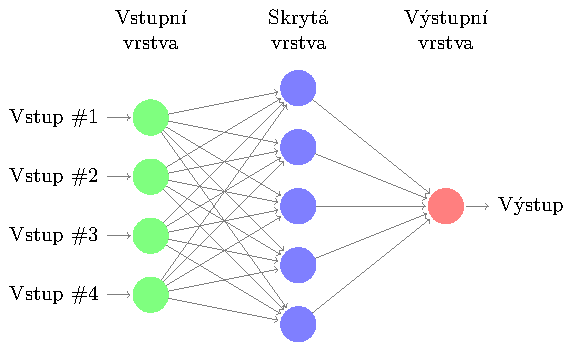
\includegraphics[width=.6\linewidth]{assets/9_ann.pdf}
\caption{Neuronová síť je propojená skupinou uzlů, podobná síti neuronů v~mozku.}
\label{fig:ann}
\end{figure}

Typickým příkladem neuronové sítě je \textbf{vícevrstvý perceptron} (ANN--MLP). Tato neuronová síť se skládá minimálně ze tří vrstev uzlů (vstupní, výstupní a~skrytou). Každý z~uzlů je \textbf{neuron}, který využívá nelineární aktivační funkci s~výjimkou vstupních uzlů:
\begin{itemize}
  \item{\textbf{Vstupní vrstva} - jedná se o~pasivní vrstvu, která nemodifikuje data, pouze je získává z~okolního světa a~pošle je dál do sítě. Počet uzlů v~této vrstvě závisí na množství příznaků nebo deskriptivních informací, které chceme extrahovat z~obrázku.}
  \item{\textbf{Skrytá vrstva} - v~této vrstvě probíhá transformace vstupů do něčeho, co může výstupní nebo jiná skrytá vrstva využít (za předpokladu, že existuje více skrytých vrstev). Počet uzlů je určen složitostí problému a~přesnosti, které chceme přidat do sítě.}
  \item{\textbf{Výstupní vrstva} - tato vrstva musí také vždy existovat v~topologii sítě, ovšem počet uzlů v~tomto případě bude definován vybranou neuronovou sítí. Pokud detekujeme na obrázku pouze jeden objekt, bude mít vrstva jen jeden uzel (lineární regrese) a~bude vracet hodnotu definující pravděpodobnost konkrétního objektu v~rozmezí $[-1,1]$.}
\end{itemize} 


\begin{itemize}
  \item Vysoká dimenze vstupního vektoru zvyšuje přesnost výsledků (ovšem zvyšuje výpočetní náklady)
  \item Aktivační funkce pro skrytou vrstvu, která umožnuje přizpůsobit nelineární hypotézy a~získat lepší detekci vzoru v~závislosti na poskytnutých datech (Sigmoid, tanh, ReLU).
  \item Hodnoty jsou získávány z~předchozí vrstvy, sečteny s~určitými váhami a~hodnotou zkreslení. (Suma těchto hodnot je transformována pomocí aktivační funkce, může se lišit pro různé neurony)
\end{itemize}

\subsubsection{Konvoluční neuronové sítě \textit{CNN} - Convolution neural network}
\begin{itemize}
  \item Speciálním druhem vícevrstvých neuronových sítí a~jsou navrženy tak, aby rozpoznaly vizuální vzory přímo z~pixelu obrazu s~minimálním předzpracováním.
  \item Mohou rozpoznat vzory s~extrémní variabilitou (například ručně psané znaky) a~odolnost vůči deformacím a~jednoduchým geometrickým transformacím.
  \item Síť využívá matematickou operaci zvanou konvoluce alespoň v~jedné jejich vrstvě.
\end{itemize}

Nejznámější a~nejvíce používanou konvoluční neuronovou sítí jsou modely LeNet.
Hlavní kroky LeNet sítě jsou:
\begin{itemize}
  \item{\textbf{Konvoluce} - tyto vrstvy provádějí konvoluci nad vstupy do neuronové sítě.}
  \item{\textbf{Nelinearita (ReLU)} - tato vrstva je použita po každé konvoluční vrstvě a~jejím cílem je nahrazení všech negativních pixelů nulou ve výstupu této vrstvy (příznaková mapa).}
  \item{\textbf{Pooling/sub sampling} - ze vstupního obrazu vyextrahuje pouze zajímavé části pomocí některých matematických operací (max, avg, sum), a~tím se redukuje jeho dimenzionalita.}
  \item{\textbf{Fully connected layer/klasifikace} - tato vrstva vychází z~původních umělých neuronových sítí, konkrétně z~vícevrstvého perceptronu. Tato vrstva je typicky umístěna na konci sítě a~je propojena s~klasifikační vrstvou pro predikci.}
\end{itemize}
\begin{figure}[H]
\centering
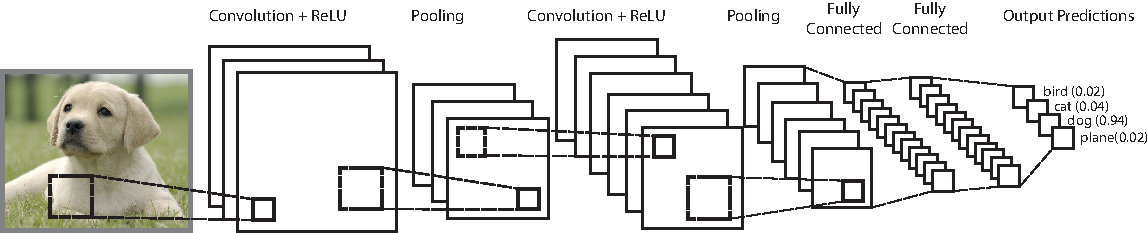
\includegraphics[width=1.1\linewidth]{assets/9_cnn.pdf}
\caption{Řetězec LeNet konvoluční neuronové sítě}
\label{fig:cnn}
\end{figure}

\subsection{Bag of words BoW}
BoW model může být aplikován pro klasifikaci obrázků, zachází s příznaky obrázků jako se slovy
\begin{enumerate}
\item Vstupem je vektor příznaků
\item centroidy z výstup k-means se stanou \uv{slovníkem}
\item poté když máme obraz, můžeme příznaku (slovu) přiřadit třídu ze slovníku
\item vytvoříme histogram počtu výskutů slov ze slovníku
\item tento histogramem dáme klasifikátoru
\end{enumerate}
